% Options for packages loaded elsewhere
% Options for packages loaded elsewhere
\PassOptionsToPackage{unicode}{hyperref}
\PassOptionsToPackage{hyphens}{url}
\PassOptionsToPackage{dvipsnames,svgnames,x11names}{xcolor}
%
\documentclass[
  11pt,
]{article}
\usepackage{xcolor}
\usepackage[margin=1in]{geometry}
\usepackage{amsmath,amssymb}
\setcounter{secnumdepth}{-\maxdimen} % remove section numbering
\usepackage{iftex}
\ifPDFTeX
  \usepackage[T1]{fontenc}
  \usepackage[utf8]{inputenc}
  \usepackage{textcomp} % provide euro and other symbols
\else % if luatex or xetex
  \usepackage{unicode-math} % this also loads fontspec
  \defaultfontfeatures{Scale=MatchLowercase}
  \defaultfontfeatures[\rmfamily]{Ligatures=TeX,Scale=1}
\fi
\usepackage{lmodern}
\ifPDFTeX\else
  % xetex/luatex font selection
\fi
% Use upquote if available, for straight quotes in verbatim environments
\IfFileExists{upquote.sty}{\usepackage{upquote}}{}
\IfFileExists{microtype.sty}{% use microtype if available
  \usepackage[]{microtype}
  \UseMicrotypeSet[protrusion]{basicmath} % disable protrusion for tt fonts
}{}
\makeatletter
\@ifundefined{KOMAClassName}{% if non-KOMA class
  \IfFileExists{parskip.sty}{%
    \usepackage{parskip}
  }{% else
    \setlength{\parindent}{0pt}
    \setlength{\parskip}{6pt plus 2pt minus 1pt}}
}{% if KOMA class
  \KOMAoptions{parskip=half}}
\makeatother
% Make \paragraph and \subparagraph free-standing
\makeatletter
\ifx\paragraph\undefined\else
  \let\oldparagraph\paragraph
  \renewcommand{\paragraph}{
    \@ifstar
      \xxxParagraphStar
      \xxxParagraphNoStar
  }
  \newcommand{\xxxParagraphStar}[1]{\oldparagraph*{#1}\mbox{}}
  \newcommand{\xxxParagraphNoStar}[1]{\oldparagraph{#1}\mbox{}}
\fi
\ifx\subparagraph\undefined\else
  \let\oldsubparagraph\subparagraph
  \renewcommand{\subparagraph}{
    \@ifstar
      \xxxSubParagraphStar
      \xxxSubParagraphNoStar
  }
  \newcommand{\xxxSubParagraphStar}[1]{\oldsubparagraph*{#1}\mbox{}}
  \newcommand{\xxxSubParagraphNoStar}[1]{\oldsubparagraph{#1}\mbox{}}
\fi
\makeatother


\usepackage{longtable,booktabs,array}
\newcounter{none} % for unnumbered tables
\usepackage{calc} % for calculating minipage widths
% Correct order of tables after \paragraph or \subparagraph
\usepackage{etoolbox}
\makeatletter
\patchcmd\longtable{\par}{\if@noskipsec\mbox{}\fi\par}{}{}
\makeatother
% Allow footnotes in longtable head/foot
\IfFileExists{footnotehyper.sty}{\usepackage{footnotehyper}}{\usepackage{footnote}}
\makesavenoteenv{longtable}
\usepackage{graphicx}
\makeatletter
\newsavebox\pandoc@box
\newcommand*\pandocbounded[1]{% scales image to fit in text height/width
  \sbox\pandoc@box{#1}%
  \Gscale@div\@tempa{\textheight}{\dimexpr\ht\pandoc@box+\dp\pandoc@box\relax}%
  \Gscale@div\@tempb{\linewidth}{\wd\pandoc@box}%
  \ifdim\@tempb\p@<\@tempa\p@\let\@tempa\@tempb\fi% select the smaller of both
  \ifdim\@tempa\p@<\p@\scalebox{\@tempa}{\usebox\pandoc@box}%
  \else\usebox{\pandoc@box}%
  \fi%
}
% Set default figure placement to htbp
\def\fps@figure{htbp}
\makeatother





\setlength{\emergencystretch}{3em} % prevent overfull lines

\providecommand{\tightlist}{%
  \setlength{\itemsep}{0pt}\setlength{\parskip}{0pt}}



 


\usepackage{amsmath,amssymb,enumitem,booktabs}
\usepackage{tikz}
\setlist{itemsep=2pt,topsep=3pt}
\usepackage{fancyhdr}\pagestyle{fancy}\fancyhf{}
\fancyhead[L]{\small DS701 Fall 2026}\fancyhead[R]{\small Homework 8}
\fancyfoot[C]{\small\thepage}
\renewcommand{\headrulewidth}{0.4pt}
\usepackage[breakable]{tcolorbox}
% --- answer-space macros (problems PDF only; no-ops in the solutions PDF) ---
% \answerspace{2in}  vertical room for handwritten work, sized from the solution
% \blank             a short fill-in rule; \blank[1.5in] for a wider one
% \answerpage        start the next problem on a fresh page (Gradescope page matching)
\newcommand{\answerspace}[1]{\par\vspace*{#1}}  % \vspace* so room is not dropped at a page break
\newcommand{\blank}[1][1.2in]{\rule{#1}{0.4pt}}
\newcommand{\answerpage}{\clearpage}
\newtcolorbox{solutionbox}{breakable,colback=blue!4,colframe=blue!45!black,title=Solution,fonttitle=\bfseries,left=4pt,right=4pt,top=3pt,bottom=3pt}
\makeatletter
\@ifpackageloaded{caption}{}{\usepackage{caption}}
\AtBeginDocument{%
\ifdefined\contentsname
  \renewcommand*\contentsname{Table of contents}
\else
  \newcommand\contentsname{Table of contents}
\fi
\ifdefined\listfigurename
  \renewcommand*\listfigurename{List of Figures}
\else
  \newcommand\listfigurename{List of Figures}
\fi
\ifdefined\listtablename
  \renewcommand*\listtablename{List of Tables}
\else
  \newcommand\listtablename{List of Tables}
\fi
\ifdefined\figurename
  \renewcommand*\figurename{Figure}
\else
  \newcommand\figurename{Figure}
\fi
\ifdefined\tablename
  \renewcommand*\tablename{Table}
\else
  \newcommand\tablename{Table}
\fi
}
\@ifpackageloaded{float}{}{\usepackage{float}}
\floatstyle{ruled}
\@ifundefined{c@chapter}{\newfloat{codelisting}{h}{lop}}{\newfloat{codelisting}{h}{lop}[chapter]}
\floatname{codelisting}{Listing}
\newcommand*\listoflistings{\listof{codelisting}{List of Listings}}
\makeatother
\makeatletter
\makeatother
\makeatletter
\@ifpackageloaded{caption}{}{\usepackage{caption}}
\@ifpackageloaded{subcaption}{}{\usepackage{subcaption}}
\makeatother
\usepackage{bookmark}
\IfFileExists{xurl.sty}{\usepackage{xurl}}{} % add URL line breaks if available
\urlstyle{same}
% fallback for those not using the hyperref driver hyperxmp:
\makeatletter
\@ifundefined{xmpquote}{\newcommand{\xmpquote}[1]{#1}}{}
\makeatother
\hypersetup{
  pdftitle={DS701 Homework 8: SVD and PCA},
  colorlinks=true,
  linkcolor={blue},
  filecolor={Maroon},
  citecolor={Blue},
  urlcolor={Blue},
  pdfcreator={LaTeX via pandoc}}


\title{DS701 Homework 8: SVD and PCA}
\usepackage{etoolbox}
\makeatletter
\providecommand{\subtitle}[1]{% add subtitle to \maketitle
  \apptocmd{\@title}{\par {\large #1 \par}}{}{}
}
\makeatother
\subtitle{Released Tue Nov 2 · due Mon Nov 9, 11:59 pm on Gradescope}
\author{}
\date{}
\begin{document}
\maketitle


\noindent\textbf{Name:}\ \rule{2.0in}{0.4pt}\qquad\textbf{BU ID:}\ \rule{1.2in}{0.4pt}
\vspace{6pt}

\textbf{How this works.} Answer \textbf{by hand on paper} (or a tablet
with a stylus), show your work, then scan and upload to Gradescope,
matching each problem to its pages. This is deliberate practice for the
closed-notes quizzes, which are in the same style --- so do it as much
as possible without a computer or an AI assistant; if stuck, try AI in
tutorial style or ask course staff. \textbf{Participation-graded:} a
serious attempt at every problem earns full credit; solutions are
released the day after the deadline. \textbf{Budget under two hours:}
seven short parts --- a concept, a reading of printed output, or one
line of arithmetic from a sheet formula; nothing decomposed by hand.

\textbf{Covers:} L12 (SVD and Low-Rank Approximation) and L13 (PCA and
t-SNE). \textbf{Reference sheet:} quiz-2 sheet §12 and quiz-3 sheet §13;
anything else is printed in the problem.

\subsection{Problem 1: Reading a singular-value
spectrum}\label{problem-1-reading-a-singular-value-spectrum}

A building has 300 temperature sensors, read hourly for 2,000 hours:
\(A \in \mathbb R^{2000\times300}\) (rows = hours, columns = sensors).
Its SVD \(A = U\Sigma V^T\) has singular values \(\sigma_1 = 40\),
\(\sigma_2 = 30\), \(\sigma_3 = 10\), \(\sigma_4 = 8\),
\(\sigma_5 = 6\), and \(\sigma_6,\ldots,\sigma_{300}\) all below
\(10^{-12}\).

\begin{enumerate}
\def\labelenumi{(\alph{enumi})}
\item
  What is the rank of \(A\)? One sentence on why the tail of tiny values
  does not count, and one on what this rank says about the 300 sensors
  (think of \(A = CR\)).

  \(\operatorname{rank} A =\) \blank[0.8in]
\end{enumerate}

\answerspace{0.4in}

\begin{enumerate}
\def\labelenumi{(\alph{enumi})}
\setcounter{enumi}{1}
\tightlist
\item
  From the spectrum alone, fill in the blanks for \(k = 1, 2, 3\). Then:
  what is the smallest \(k\) whose \(A^{(k)}\) captures at least
  \(95\%\) of \(\Vert A\Vert_F^2\), and for that \(k\), how many numbers
  does the factored \(A^{(k)}\) store, as a fraction of \(mn\)?
\end{enumerate}

fraction of \(\Vert A\Vert_F^2\) captured by \(A^{(k)}\): \(\;k{=}1\):
\blank[0.8in] \(\;k{=}2\): \blank[0.8in] \(\;k{=}3\): \blank[0.8in]

\(\Vert A - A^{(k)}\Vert_F^2\): \(\;k{=}1\): \blank[0.8in] \(\;k{=}2\):
\blank[0.8in] \(\;k{=}3\): \blank[0.8in]

\(k =\) \blank[0.6in] \(\quad\) numbers stored for \(A^{(k)}\):
\blank[0.9in] \(\quad\) fraction of \(mn\): \blank[0.9in]

\answerspace{0.3in}

\answerpage

\subsection{Problem 2: What the singular vectors
mean}\label{problem-2-what-the-singular-vectors-mean}

\emph{Practices: reading the first two singular vectors of a small table
as patterns / latent factors. Background: Appendix 12B (Reading the
Singular Vectors) works a similar example step by step.}

A café records how many of four products five regulars bought last
month:

{\def\LTcaptype{none} % do not increment counter
\begin{longtable}[]{@{}lcccc@{}}
\toprule\noalign{}
& coffee & filters & tea & honey \\
\midrule\noalign{}
\endhead
\bottomrule\noalign{}
\endlastfoot
customer 1 & 8 & 6 & 1 & 0 \\
customer 2 & 6 & 5 & 0 & 1 \\
customer 3 & 1 & 0 & 7 & 6 \\
customer 4 & 0 & 1 & 8 & 7 \\
customer 5 & 4 & 3 & 4 & 3 \\
\end{longtable}
}

Its SVD \(A = U\Sigma V^T\) has \(\sigma = (16.1,\ 12.3,\ 1.2,\ 0.8)\),
and the first two singular-vector pairs are (rounded to two decimals;
signs chosen so that \(\mathbf v_1\) is positive and the first entry of
\(\mathbf v_2\) is positive):

\[
\mathbf v_1 = \begin{bmatrix}0.45\\0.36\\0.63\\0.53\end{bmatrix}
\begin{matrix}\text{coffee}\\\text{filters}\\\text{tea}\\\text{honey}\end{matrix},
\qquad
\mathbf v_2 = \begin{bmatrix}0.65\\0.50\\-0.43\\-0.38\end{bmatrix},
\qquad
\mathbf u_1 = \begin{bmatrix}0.40\\0.31\\0.50\\0.56\\0.43\end{bmatrix}
\begin{matrix}\text{c1}\\\text{c2}\\\text{c3}\\\text{c4}\\\text{c5}\end{matrix},
\qquad
\mathbf u_2 = \begin{bmatrix}0.63\\0.49\\-0.38\\-0.46\\0.10\end{bmatrix}.
\]

\begin{enumerate}
\def\labelenumi{(\alph{enumi})}
\item
  In one sentence, what pattern in the products does \(\mathbf v_1\)
  describe, and what does a customer's entry in \(\mathbf u_1\) measure?
  Which customer has the largest first coordinate in \(U'\Sigma'\) (the
  sheet's ``row of \(U'\Sigma'\)'')? Use the printed numbers --- one
  multiplication at most.

  Customer: \blank[0.8in]
\end{enumerate}

\answerspace{1.2in}

\begin{enumerate}
\def\labelenumi{(\alph{enumi})}
\setcounter{enumi}{1}
\tightlist
\item
  Now the second pair. In one or two sentences, what \emph{contrast}
  does \(\mathbf v_2\) capture, and which customers does \(\mathbf u_2\)
  put on each side of it? What does customer 5's entry \(0.10\) say
  about them? Finally: \(\sigma_1^2+\sigma_2^2\) is \(99.5\%\) of
  \(\Vert A\Vert_F^2\) --- in one sentence, what does that tell you
  about this table?
\end{enumerate}

\answerspace{1.6in}

\answerpage

\subsection{Problem 3: PCA variance accounting, preprocessing, and a
t-SNE
map}\label{problem-3-pca-variance-accounting-preprocessing-and-a-t-sne-map}

\emph{Practices: reading eigenvalues as variances, knowing why centering
and scaling matter, and reading a t-SNE picture without over-reading
it.}

\begin{enumerate}
\def\labelenumi{(\alph{enumi})}
\tightlist
\item
  A dataset has \(m = 101\) rows and \(n = 6\) features. The features
  are \textbf{standardized} (each column centered and scaled to variance
  1) before PCA, and the covariance matrix \(S\) has eigenvalues \[
  \lambda = (3.0,\ 1.5,\ 0.9,\ 0.3,\ 0.2,\ 0.1).
  \] Fill in the table. What is the smallest number of components \(d\)
  that retains at least \(90\%\) of the variance? Why is the total \(T\)
  exactly \(6\) here, in one sentence? Lastly, if the centered,
  standardized data matrix \(X\) had been decomposed by SVD instead,
  what would \(\sigma_1\) be?
\end{enumerate}

{\def\LTcaptype{none} % do not increment counter
\begin{longtable}[]{@{}cccc@{}}
\toprule\noalign{}
PC \(i\) & \(\lambda_i\) & ratio \(\lambda_i/T\) & cumulative \\
\midrule\noalign{}
\endhead
\bottomrule\noalign{}
\endlastfoot
1 & \(3.0\) & \blank[0.8in] & \blank[0.8in] \\
2 & \(1.5\) & \blank[0.8in] & \blank[0.8in] \\
3 & \(0.9\) & \blank[0.8in] & \blank[0.8in] \\
4 & \(0.3\) & \blank[0.8in] & \blank[0.8in] \\
5 & \(0.2\) & \blank[0.8in] & \blank[0.8in] \\
6 & \(0.1\) & \blank[0.8in] & \blank[0.8in] \\
\end{longtable}
}

\(T =\) \blank[0.6in] \(\quad d =\) \blank[0.6in] \(\quad \sigma_1 =\)
\blank[0.8in]

\answerspace{1.3in}

\begin{enumerate}
\def\labelenumi{(\alph{enumi})}
\setcounter{enumi}{1}
\item
  True or false, with one reason each.

  \begin{enumerate}
  \def\labelenumii{(\roman{enumii})}
  \item
    A teammate's features are house price (dollars), age (years) and
    number of rooms. They say: ``I centered every column, so PCA is fine
    --- scaling is optional.''
  \item
    Another teammate skips centering and takes the top right singular
    vector of the raw \(X_0\) as ``PC1'': ``the top singular vector is
    the direction of maximum variance either way.''
  \end{enumerate}
\end{enumerate}

\answerspace{1.8in}

\begin{enumerate}
\def\labelenumi{(\alph{enumi})}
\setcounter{enumi}{2}
\tightlist
\item
  The figure is a t-SNE map (perplexity 30, one random start) of 100
  tissue samples, each originally described by 50 PCA features. Three
  groups are visible.
\end{enumerate}

\begin{center}
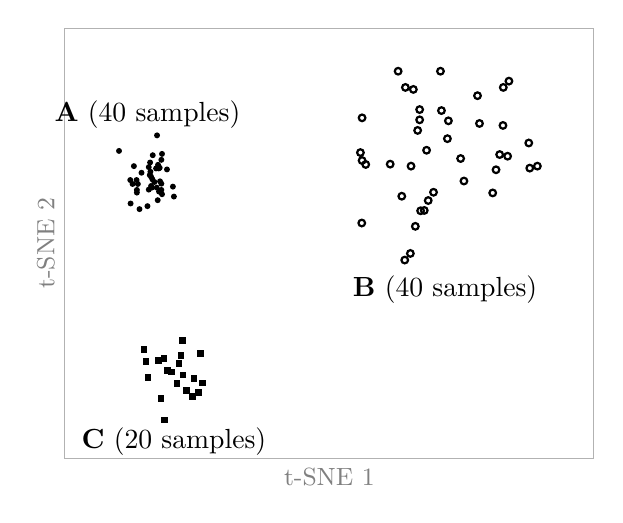
\begin{tikzpicture}[x=0.42cm,y=0.42cm]
  \def\ptsA{(-3.72,1.68),(-3.69,1.30),(-3.63,2.28),(-3.87,1.68),(-3.84,2.66),(-3.66,2.26),(-4.45,1.79),(-4.33,1.91),(-3.96,2.30),(-3.68,2.37),(-3.20,1.41),(-3.65,1.56),(-3.96,1.62),(-4.51,1.20),(-3.62,1.87),(-3.58,2.52),(-4.00,1.12),(-4.24,1.03),(-4.52,1.91),(-4.32,1.53),(-3.91,2.16),(-4.29,1.79),(-4.86,2.79),(-3.85,1.93),(-3.58,1.80),(-3.93,2.06),(-3.56,2.70),(-3.23,1.71),(-4.41,2.33),(-3.71,3.26),(-3.89,2.01),(-4.18,2.13),(-3.74,2.26),(-3.41,2.23),(-3.56,1.48),(-3.79,1.85),(-3.58,1.61),(-3.89,1.73),(-4.32,1.61),(-3.92,2.44)}
  \def\ptsB{(3.58,5.20),(4.04,4.65),(5.98,4.46),(4.89,4.01),(6.65,2.68),(3.95,-0.31),(5.47,2.56),(4.17,3.41),(6.89,2.63),(7.79,2.33),(2.60,2.38),(7.56,2.27),(7.53,3.03),(5.10,3.70),(2.49,3.79),(4.44,2.81),(5.07,3.16),(3.34,2.39),(3.69,1.42),(6.93,4.90),(6.76,4.71),(4.10,0.51),(6.75,3.56),(4.23,4.04),(4.37,0.99),(5.57,1.88),(2.48,0.61),(6.04,3.62),(2.44,2.74),(4.23,3.73),(4.65,1.54),(6.54,2.22),(4.26,0.98),(2.49,2.50),(6.44,1.52),(3.78,-0.51),(4.86,5.20),(3.97,2.33),(3.80,4.71),(4.49,1.29)}
  \def\ptsC{(-3.59,-4.70),(-2.99,-3.40),(-3.49,-5.35),(-2.33,-4.23),(-2.82,-4.45),(-4.04,-3.58),(-2.59,-4.10),(-3.05,-3.63),(-3.11,-4.25),(-3.40,-3.85),(-3.27,-3.90),(-4.11,-3.21),(-3.66,-3.54),(-3.50,-3.48),(-2.46,-4.51),(-2.94,-2.94),(-2.92,-3.99),(-3.98,-4.07),(-2.40,-3.34),(-2.63,-4.63)}
  \draw[gray!60] (-6.5,-6.5) rectangle (9.5,6.5);
  \node[below,gray] at (1.5,-6.5) {\small t-SNE 1};
  \node[rotate=90,above,gray] at (-6.5,0) {\small t-SNE 2};
  \foreach \p in \ptsA {\fill[black] \p circle (0.09);}
  \foreach \p in \ptsB {\draw[black,thick] \p circle (0.1);}
  \foreach \p in \ptsC {\fill[black] \p ++(-0.1,-0.1) rectangle ++(0.2,0.2);}
  \node at (-4.0,3.9) {\textbf{A} (40 samples)};
  \node at (5.0,-1.4) {\textbf{B} (40 samples)};
  \node at (-3.2,-6.0) {\textbf{C} (20 samples)};
\end{tikzpicture}
\end{center}

\begin{verbatim}
For each claim, say **supported** or **not supported** by this map, with one reason.

(i) "Group B's samples are more varied among themselves than group A's — look how
much more spread out B is."

(ii) "Group A is biologically closer to group C than to group B, since A sits
nearer to C."

(iii) "Two samples that sit next to each other inside group A are near neighbours
in the original 50-dimensional space."

(iv) "Re-running t-SNE with a different random seed would reproduce this layout."

Finally: the team wants to train a classifier on a 20-number summary of each
sample. Which method, PCA or t-SNE, should produce those 20 numbers, and why (one
sentence)?
\end{verbatim}

\answerspace{2.6in}




\end{document}
